%! Date = 6/4/25
\section{Motivation Plots}\label{sec:motivation-plots}
\begin{figure}[!h]
    \centering
    \begin{subfigure}{0.4\textwidth}
        \centering
        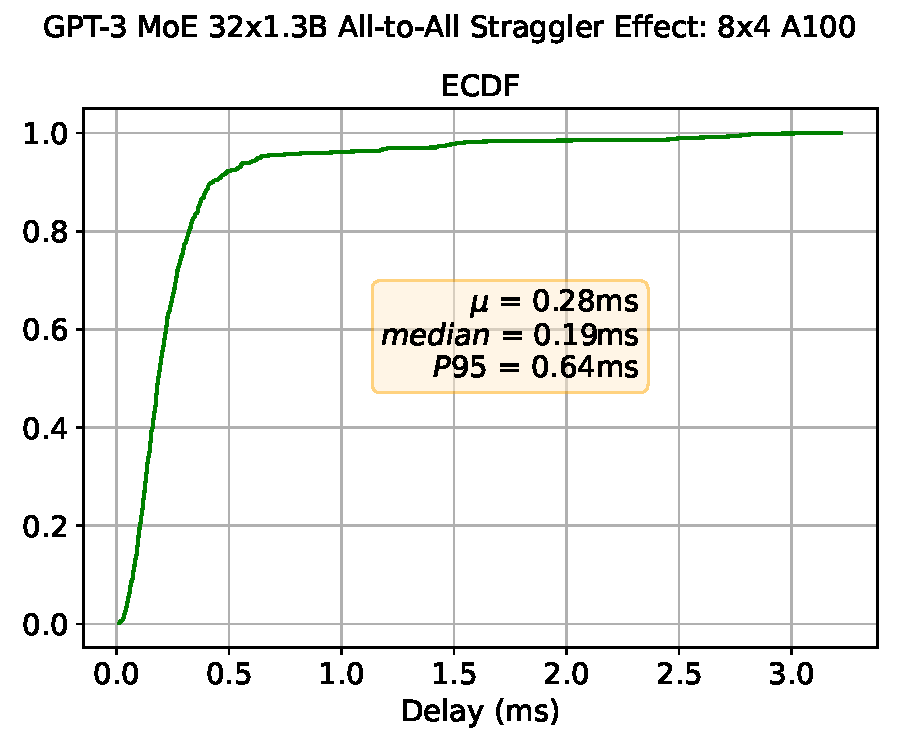
\includegraphics[width=\linewidth, keepaspectratio]{figures/GPT-3_MoE_32x1.3B_ecdf}
        \caption{ECDF}
        \label{sub:ecdf_perl}
    \end{subfigure}
    \begin{subfigure}{0.4\textwidth}
        \centering
        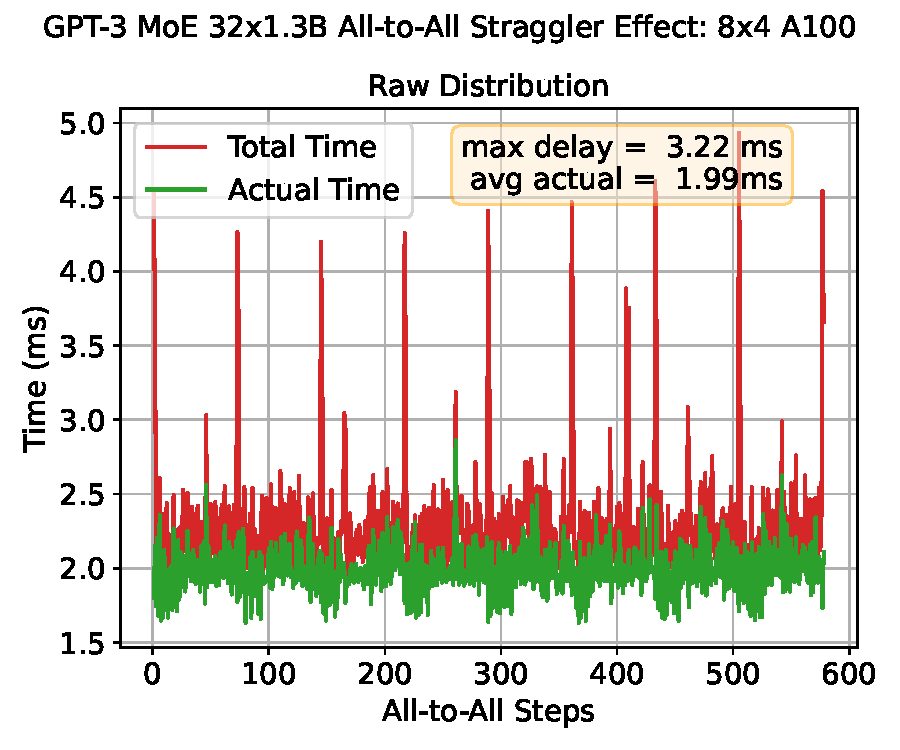
\includegraphics[width=\linewidth, keepaspectratio]{figures/GPT-3_MoE_32x1.3B}
        \caption{Raw Distribution}
        \label{sub:raw_perl}
    \end{subfigure}
    \vspace{1em} % space between rows
    \begin{subfigure}{0.4\textwidth}
        \centering
        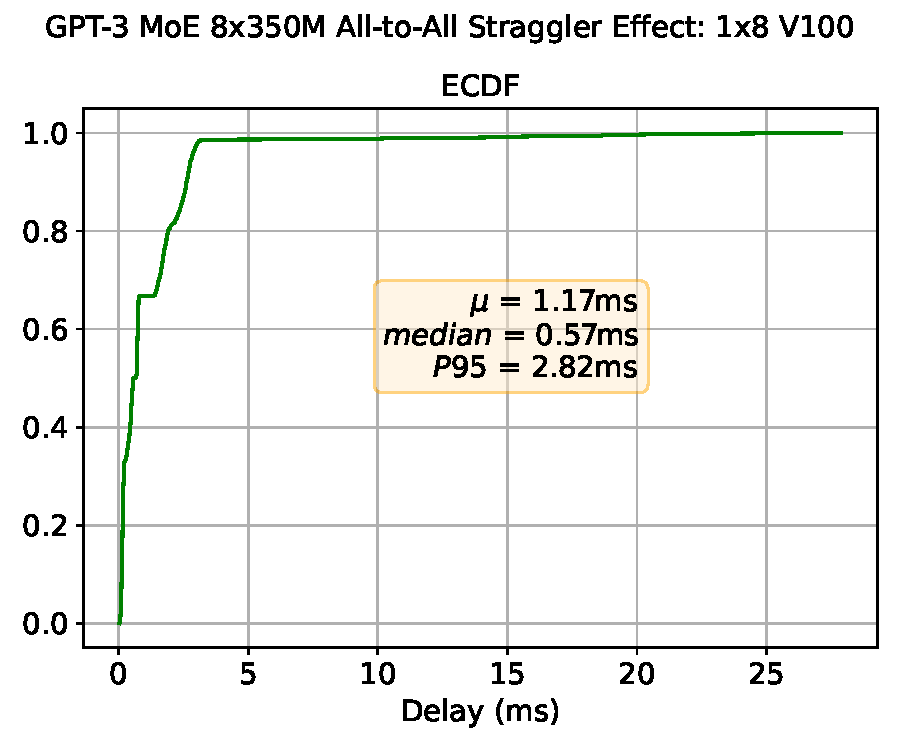
\includegraphics[width=\linewidth, keepaspectratio]{figures/GPT-3_MoE_8x350M_ecdf}
        \caption{ECDF}
        \label{sub:ecdf_az}
    \end{subfigure}
    \begin{subfigure}{0.4\textwidth}
        \centering
        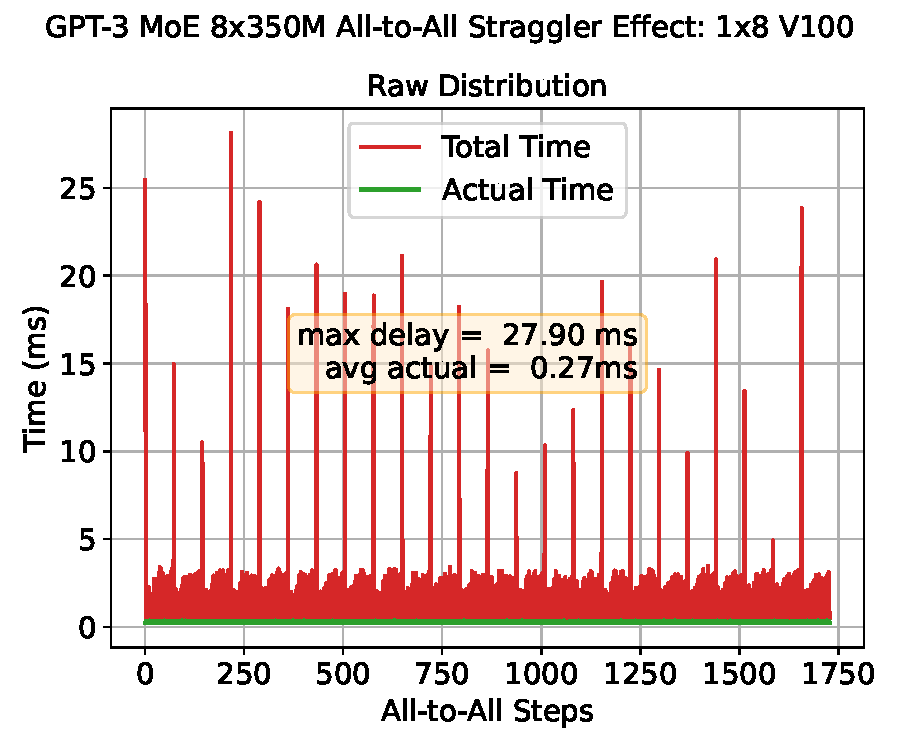
\includegraphics[width=\linewidth, keepaspectratio]{figures/GPT-3_MoE_8x350M}
        \caption{Raw Distribution}
        \label{sub:raw_az}
    \end{subfigure}
    \caption{Straggler effect of synchronous \alltoall. $M\times N$ A100 or V100 denotes
        $N$ GPUs within a node across $M$ nodes.
        Every GPU communicates with every other GPU per~\alltoall step.
        We capture the distribution of delay induced by stragglers across many steps.
        \textbf{Actual Time} $t_a$ denotes the fastest kernel execution time across all GPUs,
        conversely \textbf{Total Time} $t$ is the maximum recorded step time, while
        $Delay$ is the maximum difference between $t$ and $t_a$. Note $Delay$ is idle time.}
    \label{fig:straggler}
\end{figure}